\section{Experimental Evaluation}
\subsection{Evaluation Goals}
In this section we experimentally evaluate  Crypt$\epsilon$ to assess its practical utility  based on two parameters, the accuracy and the performance of the Crypt$\epsilon$ programs. Specifically the experiments were designed to answer the following questions:
\begin{enumerate}\item Does Crypt$\epsilon$ programs have constant error bounds depending only on the privacy parameter $\epsilon$  which is at least $O(\sqrt{m})$ times lower than that for the corresponding state-of-the-art LDP implementation? \item Is the program execution timings for Crypt$\epsilon$ practical? \item Does the proposed DP- optimizations provide substantial performance improvement over the base case Crypt$\epsilon$ implementation? \end{enumerate}
%\textit{Evaluation Highligts:}
\subsection{Methodology} 
\textbf{Programs:}
To answer the aforementioned questions we ran the experiments on the 7 Crypt$\epsilon$ programs previously outlined in section 5. Each program is compared with the corresponding state-of-the-art \textsf{LDP} implementations. %\begin{itemize}\item \textbf{Program 1} - Count the number of records having age in range $[50,60]$ \\\textbf{\textsf{LDP} Competitor} - Frequency oracle of \cite{LDP1} constructed over attribute $Age$. \item \textbf{Program 2} - Report the top 5 most frequent age values. \\\textbf{\textsf{LDP} Competitor} - Frequency oracle of \cite{LDP1} constructed over attribute $Age$.  \item \textbf{Program 3 }- Report the marginal on attributes $Age$ and $Gender$. \\\textbf{\textsf{LDP} Competitor }- Frequency oracle of \cite{LDP1} constructed over attribute $Age \times Gender$. \item \textbf{Program 4 }- Report the marginal on attributes $Age$ and $Gender$ with $NativeCountry=Mexico$\\\textbf{\textsf{LDP} Competitor }- Frequency oracle of \cite{LDP1} constructed over attribute $Age\times Gender \times NativeCountry$. \item \textbf{Program 5 }- Count the number of natively Mexican male employees of age 30.\\\textbf{\textsf{LDP} Competitor }- Frequency oracle of \cite{LDP1} constructed over attribute $Age\times Gender \times NativeCountry$. \item \textbf{Program 6 }- Count the number of distinct age values for male employees. \\\textbf{\textsf{LDP} Competitor }-Frequency oracle of \cite{LDP1} constructed over attribute $Age\times Gender$.% and reports the number of non-zero counts after suitable adjustment for thresholding. 
%\item \textbf{Program 7 }- Count the number of age values with at least 10 records. \\\textbf{\textsf{LDP} Competitor }- Frequency oracle of \cite{LDP1} constructed over attribute $Age$. \end{itemize}
\\\textbf{Datasets:}
We ran our experiments on a dataset which is generated from the UCI Adult dataset by randomly sampling 1000 records. The experiment numbers are reported as the mean value after 10 repetitions.
\\\textbf{Metrics:}
\\\textit{Accuracy:} For accuracy the following metrics are used
\begin{itemize}\item Programs 1, 6 and 7 use absolute error $ =|C-\hat{C}|$ where $C$ is the true count and $\hat{C}$ is the noisy  output. \item Program 2 uses the error measure given by the fraction of age values returned in the top 5 that have value less than $ct_5-\alpha$  where  $ct_5$ is the count of the $5^{th}$ largest value and $\alpha=\frac{1}{\epsilon}\log\frac{1}{\delta}$ is a slack parameter. The slack parameter is required because with probability $1-\delta$ no differentially private algorithm can distinguish between any two counts that differ by less than $\alpha$. We use $\delta=0.05$ for our experiment. \item Programs 3, 4 and 5 uses the $L1-Norm$ error metric given  by $Error=\sum_{i}|C[i]-\hat{C}[i]|, i \in [|C|]$ \end{itemize}
\textit{Performance:} For measuring performance we report the total execution time in seconds for each program.
\subsection{End-to-End Evaluation}
\subsubsection{Accuracy}
There are two main observations in terms of the accuracy.
The first observation is that the error for a single frequency counting program for the base case Crypt$\epsilon$ implementation is of the order $O(\frac{1}{\epsilon})$. In fact it quantitatively approximates $\frac{2}{\epsilon}$. This is in cohorts with our expectation as we add two instances of Laplace noise at the \textsf{AS} and the \textsf{CSP} and s.t.d of $Lap(\frac{1}{\epsilon})$ is given by $\frac{1}{\epsilon}$. For e.g., in Figure 2a we observe that for Program 1 error is $17.60$ for $\epsilon=0.1$ and   error is $0.1$ for $\epsilon=1.9$. Figure 2c shows that for Program 3 the errors for Crypt$\epsilon$ is approximately $200\cdot\frac{2}{\epsilon}$ (error is $4016.7$ for $\epsilon=0.1$, error is $1330.4$ for $\epsilon=0.3$). It is so because, the attribute $Age$ has domain size $100$ while attribute $Gender$ is of size $2$. Hence $Age\times Gender$ is of domain size $200$. Similarly for Program 4 in Figure 2d, the error is again around $\frac{2}{\epsilon}$ ($\epsilon=0.1$ gives error $4032.4$).  For Program 5 again, Figure 2e shows that  $\epsilon=0.1$ results in error equal to $21.8$ while for $\epsilon=1.9$ we get an error of only $0.3$. \par 
In contrast, the error corresponding to the $\textsf{LDP}$ implementation is of the order $O(\frac{\sqrt{m}}{\epsilon})$. For Program 1, we observe in Figure 2a that the error values are at least $300 >\frac{11}{2}\cdot \sqrt{m}=  \frac{11}{2}\cdot \sqrt{1000} \approx 176$ times worse. This observation is intuitive as for answering Program 1 we need to read $11$  counts from the frequency oracle (for the range [50,60]) and the factor of $\frac{1}{2}$ comes from the fact that the errors in Crypt$\epsilon$ are roughly $\frac{2}{\epsilon}$. For e.g., the error for $\textsf{LDP}$ is $967 \times$  higher than that of Crypt$\epsilon$ for $\epsilon=1.9$. For Program 3 and Program 4, we observe in Figure 2c and 2d respectively that the error values of the $\textsf{LDP}$ implementation is at least $18 >\frac{\sqrt{m}}{2}=16 $ times higher than that of base case Crypt$\epsilon$. For e.g., $\epsilon=0.1$ results in almost $25 \times$ higher errors for both programs for the respective \textsf{LDP} implementations. Similarly as seen Figure 2e, Program 5 also has at least $25\times$ worse errors for the \textsf{LDP} implementation. 
\par
Programs 2, 6 and 7 do not report counts of records in the database directly but some statistics based on the counts. Even here we observe that the accuracy of Crypt$\epsilon$ is significantly higher than that of the corresponding \textsf{LDP} implementations. For e.g., for Program 2 Figure 2b shows that on an average with $\epsilon=0.1$ Crypt$\epsilon$ can correctly identify at least 2 out of the 5 most frequent age values while the \textsf{LDP} implementation can identify none at all.  For Program 6, from Figure 2f we observe that the error values for Crypt$\epsilon$ is at least $38.5 \times$ less than that for the \textsf{LDP} implementation. The true count for distinct ages for male employees for our experimental setup happens to be $47$. Thus for $\epsilon=0.1$ the relative error ( $\frac{|C-\hat{C}|}{C}$) for the base case Crypt$\epsilon$ implementation is given by  $0.4$ while \textsf{LDP} has error $1.2$. Similarly from Figure 2g we observe for Program 7 that for $\epsilon=0.3$ the error for Crypt$\epsilon$ is $6.7$ while that for the \textsf{LDP} implementation is $26.2$. The true non-noisy answer for this program in our experimental setup is $38$. Thus the relative error $(\frac{|C-\hat{C}|}{C})$ for Crypt$\epsilon$ is $0.18$ as compared to that of $0.69$ for the \textsf{LDP} implementation.  For $\epsilon=1.9$, Crypt$\epsilon$ gives an error of just $0.5$. In contrast,  for the corresponding \textsf{LDP} implementation we still get an error of $10.6$. 
\subsubsection{Performance}
In Table 2 we report the execution time of  the aforementioned $7$ Crypt$\epsilon$ programs. For Program 1 we see that the total time taken for execution for the base case Crypt$\epsilon$ implementation is about 0.5 seconds; the cost is mainly dominated by the \textsf{AS} which has to make a pass through the entire encrypted database. The \textsf{CSP} on the other hand is just needed for decryption in the last step. Program 2 needs to compute the encrypted $Age$ histogram via $GroupBy*$ primitive which takes about $6$ seconds. The \textsf{CSP} time is also more than the previous case because of the garbled circuit in the $NoisyMax$ primitive. The total execution time for the base case implementation for Program 3 is roughly 2 hours.  The reason behind this comparatively higher timing as compared to that of the previous two programs is that the \textsf{CrossProduct} primitive requires  multiplication of the ciphers  which is costlier than the addition operator $\bigoplus$. For Program 4, we observe that the base case implementation takes around 3.1 hours to run. The timing is greater than that for Program 3 because, in this case the additional condition $NativeCountry=Mexico$ results in extra interactions with the \textsf{CSP}. Program 5 requires about $35$ seconds to execute in the base case while Program 6 runs for $41$ minutes. For Program 7 we see that the majority of the time is required by the \textsf{CSP} for generating the encrypted one-hot-codings for the $GroupBy$ primitive and takes $24$ minutes to execute.  An important observation throughout the experiments is that the time taken by the \textsf{AS} is significantly greater than that for the \textsf{CSP} for all the programs except for Program 7. This is a desirable trait for Crypt$\epsilon$ as discussed in section 3.6.
\subsection{Optimization Evaluation}
\subsubsection{Accuracy}
\textbf{\textit{\\Index}}- Programs 4, 5 and 6 can be optimized by the construction of a differentially private index. Programs 4 and 5 construct the index over the attribute $NativeCountry$ while Program 6 indexes over attribute $Gender$.  For our experiments we use $\epsilon=1$ for constructing the index. Thus in figures 2d, 2e and 2f, a privacy parameter $\epsilon=1.1$ for the optimized Crypt$\epsilon$ implementation means that $\epsilon=1$ is invested in the  index construction while $0.1$ is expended in the subsequent count. The accuracy of the differentially private index optimization is lower than that of the base case Crypt$\epsilon$ implementation. It is so because for $\phi=(A==v)$ the noisy index over $A$ might miss some of the records having value $v$ for attribute $A$, thereby introducing additional errors. However the errors are still significantly better than that of the corresponding \textsf{LDP} implementations. For e.g., as seen in Figure 2d for Program 4 the accuracy of the optimized Crypt$\epsilon$ implementation is $2.8\times$ lower for $\epsilon=1.9$ than that of the base case. However, it is still $4.8 \times$ higher than that of the corresponding \textsf{LDP} implementation.  Figure 2e shows that for Program 5 the error values for the optimized implementations of Crypt$\epsilon$  is at most $18.8 \times$ worse than that of the base case and at least $2\times$ better than that of the \textsf{LDP} implementation. For Program 6, from Figure 3f we see that the error for the optimized Crypt$\epsilon$ implementation falls drastically with $\epsilon$; for $\epsilon=1.9$ the error value is just $6\times$ higher than that of the base case implementation. It is so because the index is constructed over attribute $Gender$ and the program selects the rows corresponding to male employees. Thus even if some of the rows for male employees get missed due to the noisy index, it is highly unlikely that those missed rows will be having a new age value that does not appear in the rows selected noisily.
\\\\\textit{\textbf{Range Tree}} - Programs 1 and 2 can benefit from a range tree constructed over attribute $Age$. For Program 1, the range query for age in $[50,60]$ can be directly answered from the range tree while for Program 2, the optimized implementation reads of the values of all the leaves in  the range tree (each leaf corresponds to the count of a single age value) instead of the \textsf{GroupBy*} primitive. For Program 1, as seen from Figure 2a, the accuracy of the range tree based Crypt$\epsilon$ implementation is poorer as compared to that of the base case. For e.g., for $\epsilon=0.3$, the error for the optimized implementation is $25.2$ while that for the base case is $5$. This is so because the sensitivity of the range tree is $\log k$ where $k$ is the number of leaves (100 in this case) and a range query can take up to $2 \log k$ nodes for answering. Thus for a single query, the base case implementation will give better accuracy results. The accuracy gain for range trees kicks in for answering multiple range queries as showcased in Figure 3h.  For this experiment we execute 100 random range queries and report the sum of the absolute errors $\sum_{i=1}^100|C_i-\hat{C}_i|$ where $C_i$ is the true count of the $i^{th}$ query and $\hat{C}_i$ is the corresponding noisy value. The $\epsilon$ values reported is the total privacy budget for the $100$ queries. We observe that the error for the base case is of the order $O\big(2\cdot100\cdot\frac{100}{\epsilon}\big)$ whereas the error for the optimized implementation is at least $16 > \frac{100}{(\log k)^2}\approx 2 $ times lower.  For e.g., $\epsilon=9$ results in error=$1637$ for base case Crypt$\epsilon$ whereas the optimized implementation has error=$60$ only. In contrast the \textsf{LDP} implementation has at least $300\times$ higher error. It is so because firstly \textsf{LDP} has an additional $\sqrt{m}$ factor, secondly for answering a range query for $[r,r+t]$ in the \textsf{LDP} implementation, we have to read $t$ separate noisy counts which augments the error. For instance, for $\epsilon=0.1$, \textsf{LDP}'s error is $538500.73$. \begin{table}[ht]
\caption{Execution Time Analysis for Crypt$\epsilon$ Programs}
\centering
\begin{tabular}{c c c c c c}
\toprule
Program &  \multicolumn{3}{c}{Base} & \multicolumn{2}{c}{Optimized} \\ 
 & AS &  CSP & Total & Total & Speed up  \\ &(s)&(s)&(s)&(s)&$\times$\\ % inserts table %heading
\midrule
1 & 0.49& 0.0027& 0.4927 & 0.0029 & 168.9 \\
2 &  6.12 & 0.3  &6.42 & 0.89 & 7.2\\ %197 the communication rounds
3&  3859.52 & 3661.29 & 7520.81&N/A&N/A \\4  &7765.16&3624.05&11389.21& 910.96 & 12.5 \\5&18.56&16.7&35.26&3.49 & 10.1 \\6&1910.01&571.11&2481.12&429.92 & 5.77\\7&6.35 & 1393.89 & 1400.24 &  N/A & N/A \\ [1ex]
\bottomrule
\end{tabular}
\label{c}
\end{table}
\subsubsection{Performance}
\begin{figure}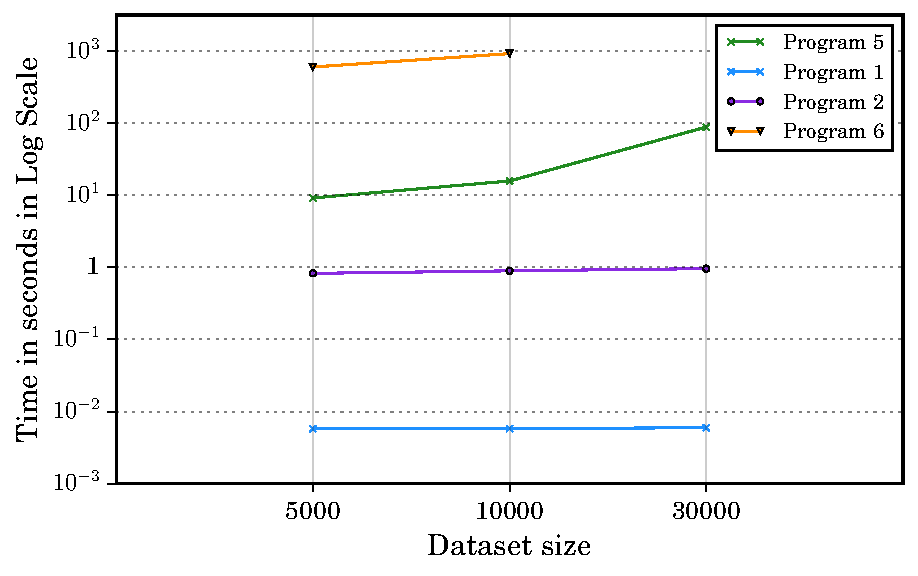
\includegraphics[width=5cm,height=3.1cm]{scalet.pdf} \caption{ Crypt$\epsilon$ Program Scalability} \end{figure}
\textit{\textbf{\\Index}}-For Program 4, we observe that the base case implementation takes around 3.1 hours to run. However the  index optimization reduces the execution time to about $15$ minutes  giving us a $12.5\times $ speedup. It is so because, only 11\% of the data records satisfy $NativeCountry$=Mexico. Thus the index reduces the number of records to be considered for the dataset drastically thereby resulting in s huge performance boost. Similarly for Program 5 again the DP index optimization results in a $10\times$ speedup with the total running time being less than $4$ seconds. For Program 6 the DP index is constructed over attribute $Gender$. While the base case takes about 40 minutes to execute, the optimized code needs only 7 minutes to run thereby reducing the time  $5.7\times$.\\\\\textit{\textbf{Range Tree}}
 For Program 1 we see that the total time taken for execution for the base case Crypt$\epsilon$ implementation is about 0.5 seconds while using the range tree optimization we get a $138\times$ speed up in timings. Note that the time required by the \textsf{AS} becomes almost negligible because it just simply needs to do a memory fetch to read of the answer from the pre-computed range tree instead of computing it from the entire encrypted database. The time for the \textsf{CSP} remains the same in both the cases, it is the decryption cost. For Program 2, we observe a $7\times$ performance improvement with the range tree optimization. Again, the reason is even in this case the \textsf{AS} can simply read off the leaf nodes of the range tree instead of computing their counts from the database. 
\begin{figure*}
    \centering
    \begin{subfigure}[b]{0.2\textwidth}
        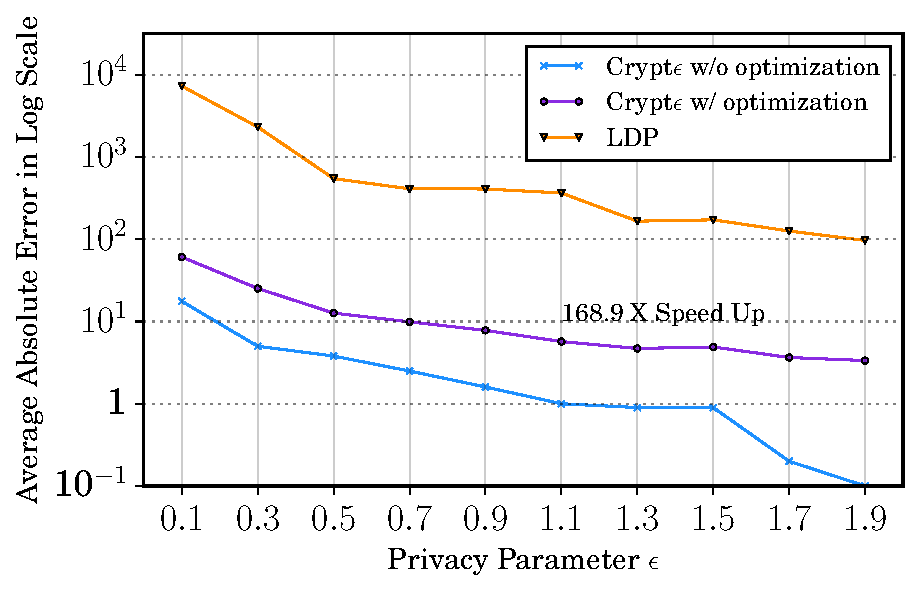
\includegraphics[width=5cm,height=3.1cm]{t1.pdf}
        \caption{ Program 1}
        \label{fig:gull}
    \end{subfigure}\quad \qquad\quad 
    ~ %add desired spacing between images, e. g. ~, \quad, \qquad etc.
      %(or a blank line to force the subfigure onto a new line)
    \begin{subfigure}[b]{0.3\textwidth}
       \qquad 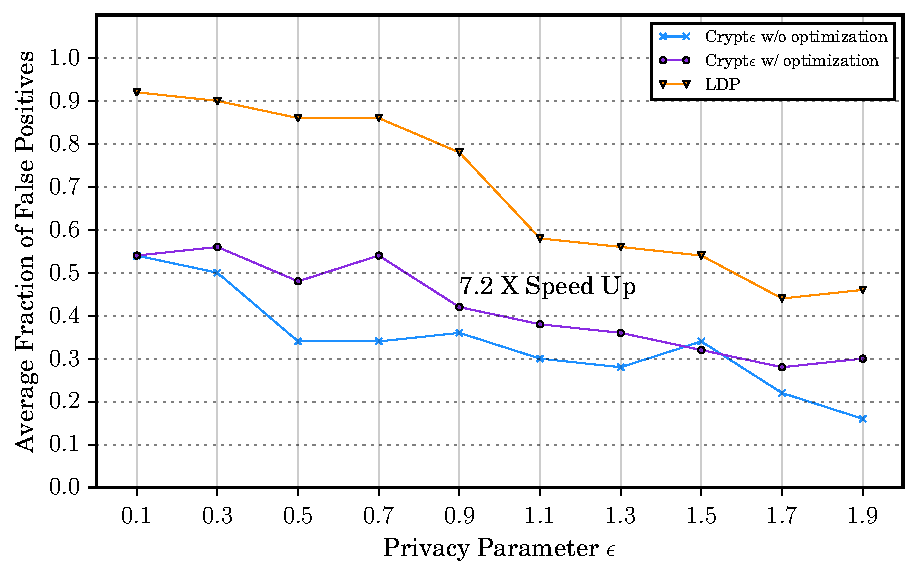
\includegraphics[width=5cm,height=3.1cm]{t22.pdf}
        \caption{ Program 2}
        \label{fig:tiger}
    \end{subfigure}
    ~ %add desired spacing between images, e. g. ~, \quad, \qquad etc.
      %(or a blank line to force the subfigure onto a new line)
    \begin{subfigure}[b]{0.3\textwidth}
    \qquad    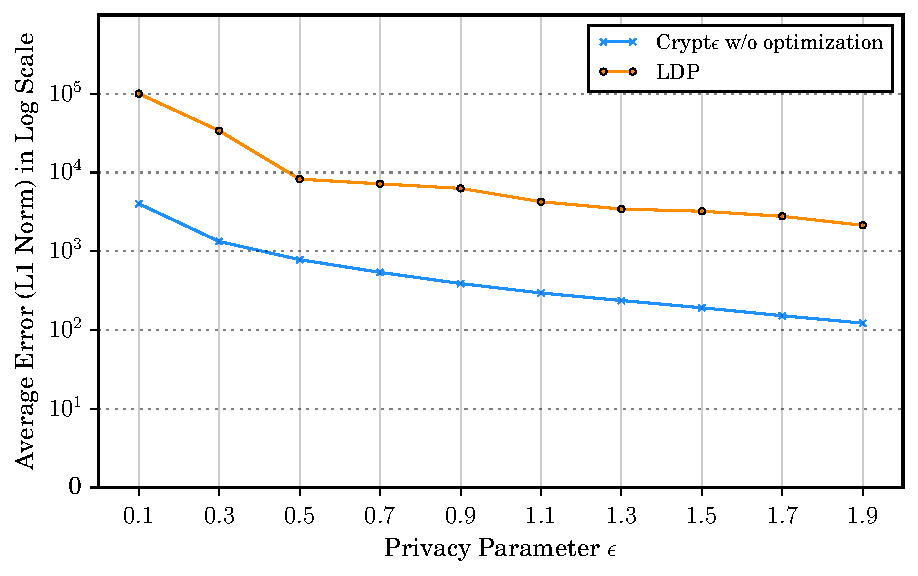
\includegraphics[width=5cm,height=3.1cm]{t3.pdf}
        \caption{Program 3}
        \label{fig:mouse}\end{subfigure}
          \begin{subfigure}[b]{0.3\textwidth}
    \qquad    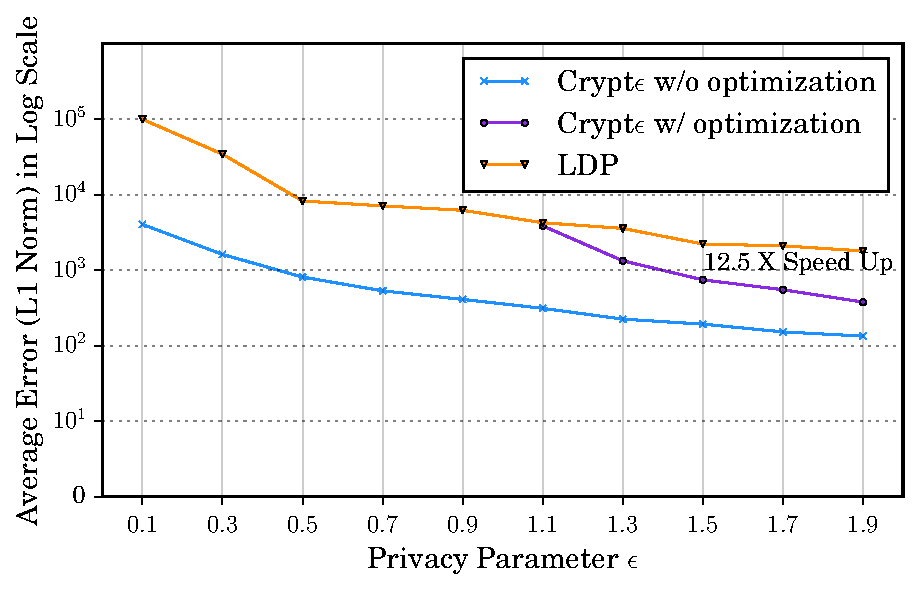
\includegraphics[width=5cm,height=3.1cm]{t4.pdf}
        \caption{Program 4}
        \label{fig:mouse}\end{subfigure}
          \begin{subfigure}[b]{0.3\textwidth}
    \qquad    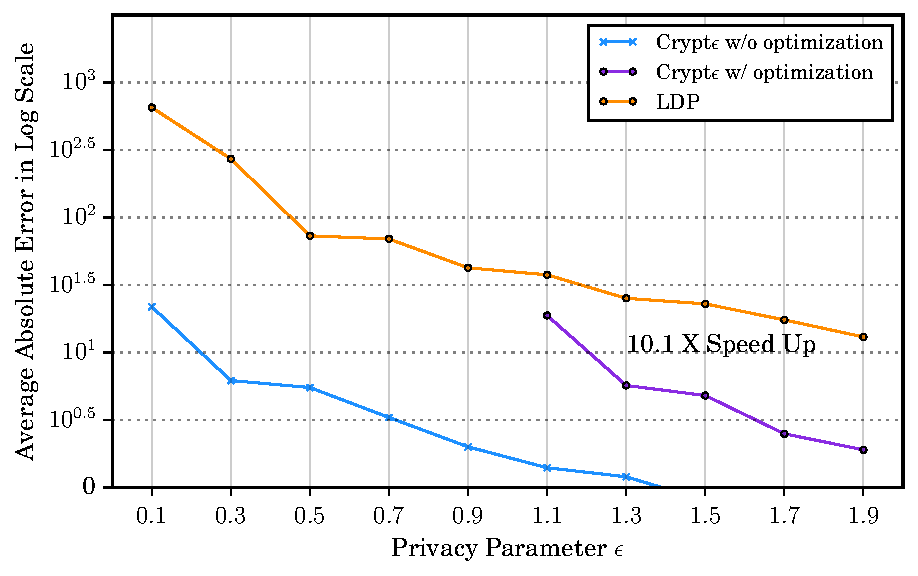
\includegraphics[width=5cm,height=3.1cm]{t5.pdf}
        \caption{Program 5}
        \label{fig:mouse}\end{subfigure}
          \begin{subfigure}[b]{0.3\textwidth}
    \qquad    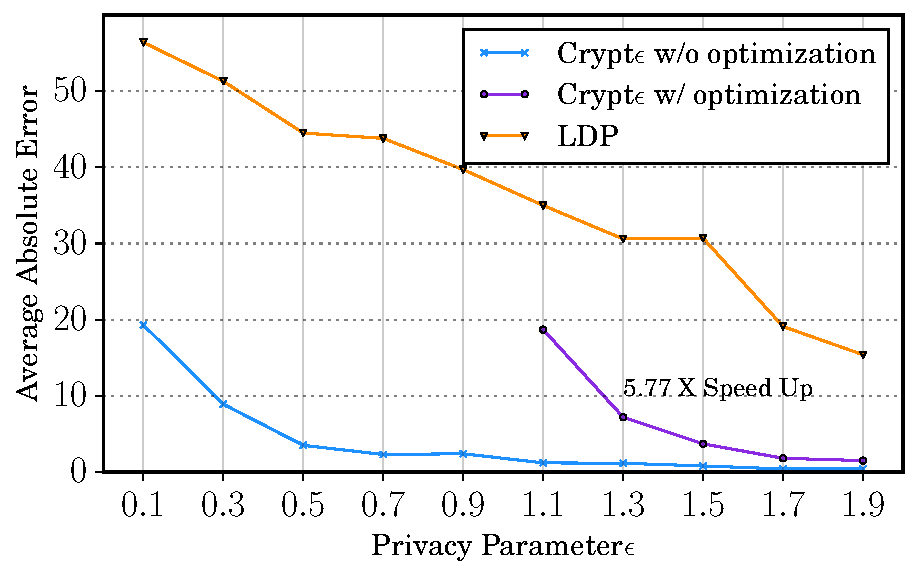
\includegraphics[width=5cm,height=3.1cm]{t6.pdf}
        \caption{Program 6}
        \label{fig:mouse}\end{subfigure}
          \begin{subfigure}[b]{0.3\textwidth}
    \qquad    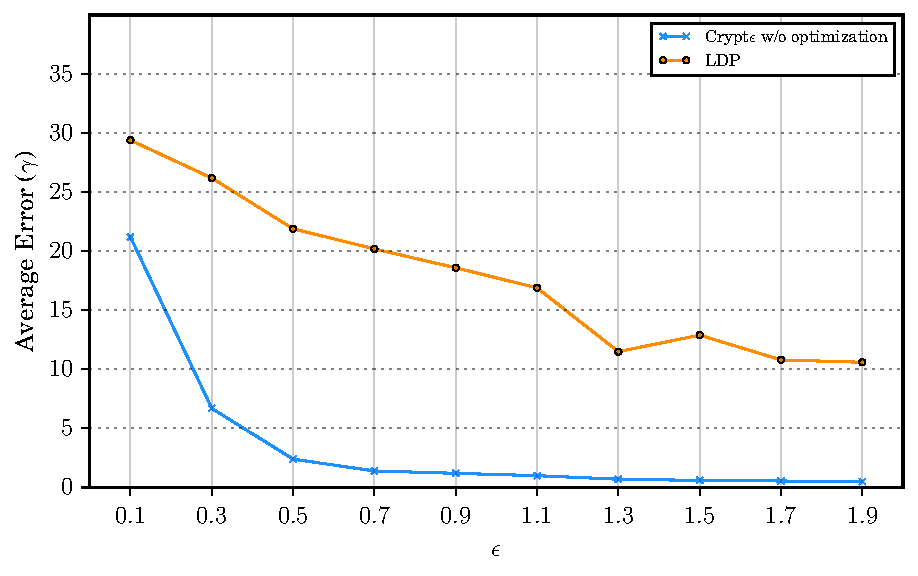
\includegraphics[width=5cm,height=3.1cm]{test7.pdf}
        \caption{Program 7}
        \label{fig:mouse}
    \end{subfigure}
    \begin{subfigure}[b]{0.3\textwidth}
    \qquad    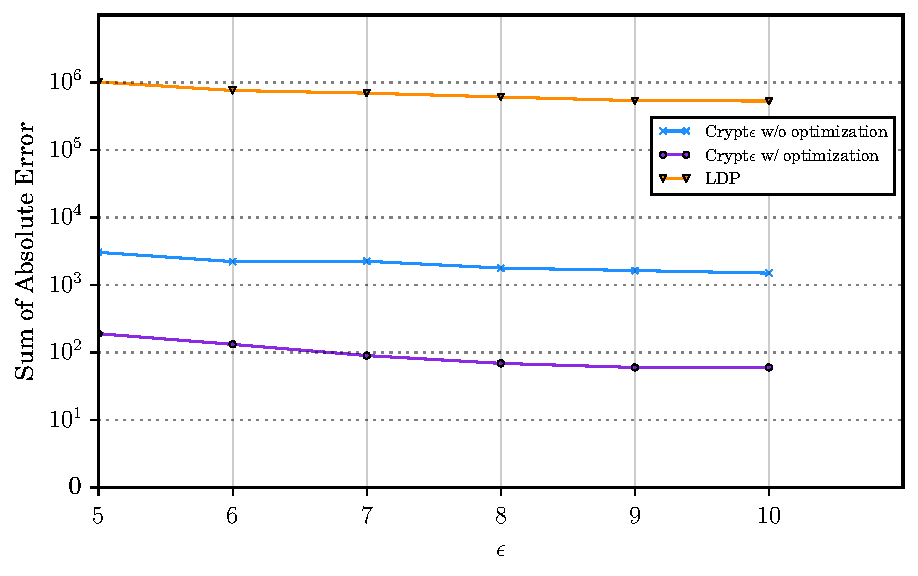
\includegraphics[width=5cm,height=3.1cm]{range.pdf}
        \caption{100 random range query evaluation}
        \label{rangetree}
        \end{subfigure}
        \begin{subfigure}[b]{0.3\textwidth}
       \qquad 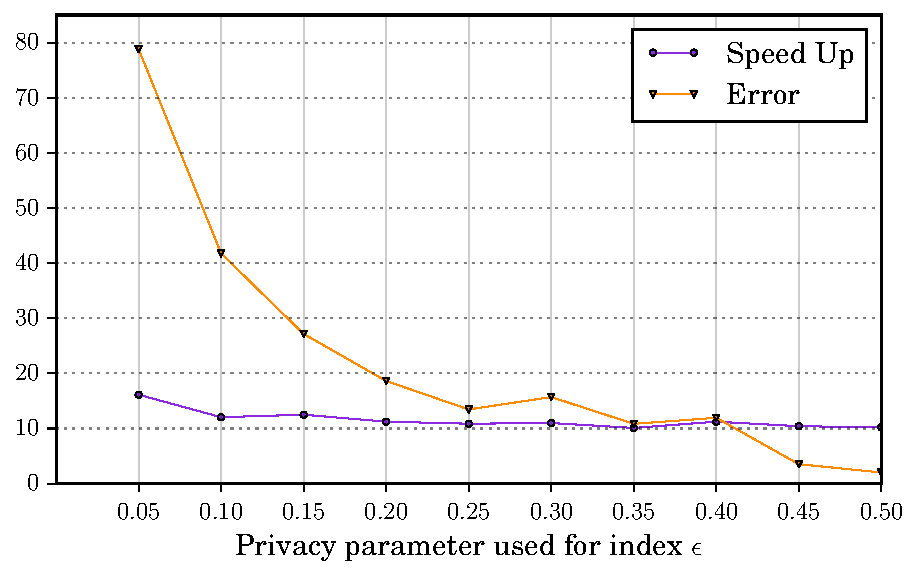
\includegraphics[width=5cm,height=3.1cm]{index.pdf}
        \caption{Privacy Budget analysis for Index Optimization}
        \label{rangetree}
    \end{subfigure}
%    \caption{a) External alignment is the neighborhood of read $X$ in the full genome and $\lambda$ is the \% of $X$ that correctly identifies it. (b) Internal alignment is the index-to-index alignment within the neighborhood of $X$ and $\sigma=avg_i\frac{TBScore_{opt}-TBScore_i}{TBScore_{opt}}$ where $TBScore_{i}=\sum_{[i,j] \in \textit{Traceback path}}\mathbf{M}[i,j]$. 
%   (c) $\rho$ is the number of reads required to cover a single index such that Pr( SNPs are aligned correctly in $Y) > 0.95$}
   \caption{Accuracy Analysis of Crypt$\epsilon$ Programs}
\end{figure*}




\paragraph{\textbf{Note:}} We observe that in Crypt$\epsilon$ we add two separate instances of the Laplace noise as opposed just one instance of noise in the traditional \textsf{CDP} setting. Thus although the errors of both Crypt$\epsilon$ and \textsf{CDP} are of the same order $O\big(\frac{1}{\epsilon}\big)$, yet quantitatively the error values of Crypt$\epsilon$ are twice that of the traditional $\textsf{CDP}$ setting. This can be addressed by a joint computation of a single instance of noise by both \textsf{AS} and \textsf{CSP} as discussed in section 9.1. Another observation is that this double noise addition does not affect the differential privacy guarantee. After the addition of the first instance of noise by the \textsf{AS}, the second can be seen as a post-processing step and differential privacy is post-processing immune. Hence our results Crypt$\epsilon$ programs are still differentially private.


